\section{Simulation mit MATLAB}

%-------------------------------------------------------------------------------
%
% Aliasing
%
%-------------------------------------------------------------------------------
\subsection{Aliasing}
\subsubsection{Aufgabenstellung}
\begin{enumerate}
\item Wählen sie Frequenz und Abtastfrequenz so, dass eine Aliasingfrequenz von $440$Hz auftritt. Überprüfen sie das Resultat graphisch und akustisch (Klavier).
\item Erzeugen Sie einen Frequenzsweep, bei dessen Abtastung Aliasing auftritt. Wählen Sie als Anfangsfrequenz eine Frequenz im Hörfrequenzbereich, und als Endfrequenz eine Frequenz um $3 \cdot f_c$. \\
Überprüfen Sie das Resultat graphisch (sowohl im Zeitbereich als auch im Frequenzbereich) und akustisch. 
\item Wählen Sie die Datei ``Flöte'' aus. Durch Eingabe einer neuen Samplingfrequenz ($44100/L$, wobei $L$ ganzzahlig sein muss), kann das eingelesene Audiosignal ohne Bandbegrenzung unterabgetastet werden. Schätzen Sie die Auswirkungen ab. Überprüfen sie akustisch die Auswirkungen des Downsamplings ohne Einhaltung des Abtasttheorems. Ab welcher Frequenz werden Aliasing Effekte hörbar? Wodurch ergibt sich diese Frequenz?
\end{enumerate}



\subsubsection{Tabellen}
Es wurden keine Tabellen benötigt.

\subsubsection{Formeln}
Berechnung der Signalfrequenz $f_S$ in Abhängigkeit von der Abtastfrequenz und der gewollten Aliasingfrequenz:
\begin{equation}\label{eq:1_1}
 f_S = |f_C - f_a|
\end{equation}

\subsubsection{Berechnungsbeispiele}
Berechnung der Signalfrequenz $f_S$ bei einer Abtastfrequenz $f_C = 44100Hz$ und einer auftretenden Aliasingfrequenz von $f_a = 440Hz$:
\begin{equation}
 f_S = |f_C - f_a| = |44100Hz - 440Hz| = 43660Hz
\end{equation}
\pagebreak

\subsubsection{Diagramme}
\begin{figure}[h!]
\centering
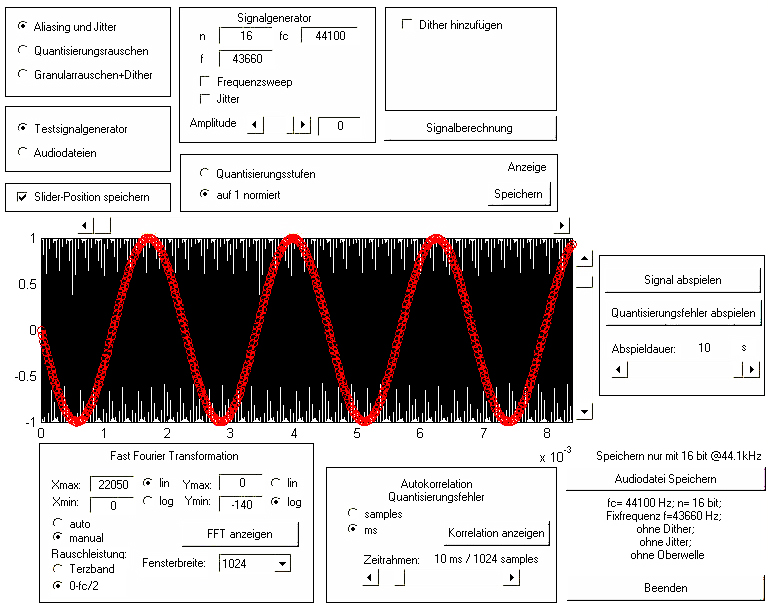
\includegraphics[width=\columnwidth]{figures/Aufg1/1_1.JPG} 
\caption{Grafische Darstellung der Aliasingfrequenz $f_a$ im Simulationsprogramm ``Störverhalten".}
\end{figure}

\begin{figure}[h!]
\centering
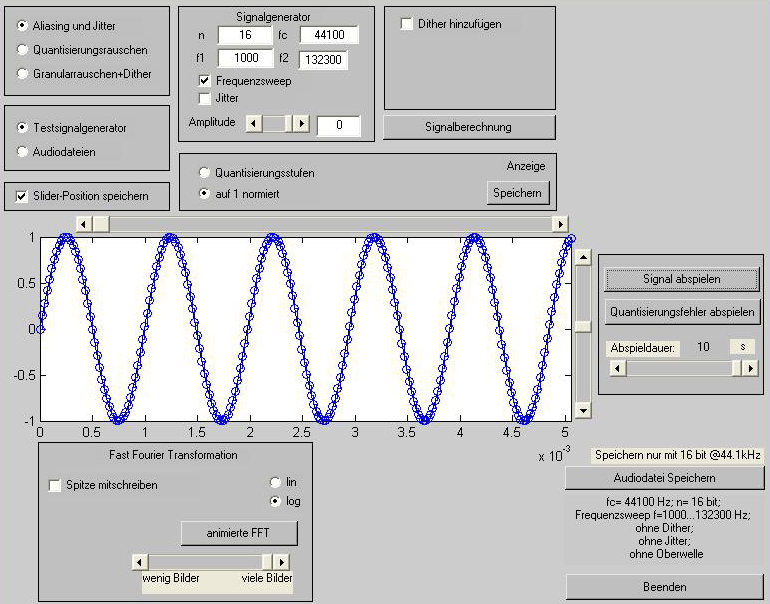
\includegraphics[width=\columnwidth]{figures/Aufg1/1_2.JPG} 
\caption{Darstellung eines Teiles (ohne Aliasing) des Frequenzsweep von 1000Hz bis $3 \cdot f_C = 132300$Hz im Simulationsprogramm ``Störverhalten".}
\end{figure}

\clearpage

\subsubsection{Diskussion}
Um, wie in Aufgabe 1 gefordert, eine Frequenz von $f_a = 440Hz$ mittels Aliasing zu erzeugen muss eine Signalfrequenz $f_S$ mit einem Abstand von $f_a$ zur Abtastfrequenz $f_C$ verwendet werden. Dieser Zusammenhang wird von der Formel (\ref{eq:1_1}) beschrieben und führte mit den gegebenen Werten zu $f_S = 43660Hz$. Tastet man dieses Signal nun mit $f_C$ ab, wird das Signal um jedes Vielfache von $f_C$ gespiegelt. Deswegen tritt auch bei 440Hz eine Spiegelung des ursprünglichen Signals auf. Dieses Aliasingsignal wurde abgespielt und entsprach der Note $a^1$ auf dem Klavier.\\
\\
In Aufgabe 2 wurde die Anfangsfrequenz des Frequenzsweep mit 1000Hz gewählt. Die Endfrequenz ergabt sich mit der Angabe $3 \cdot f_C$ zu 132300Hz. Dieser Frequenzsweep wurde über Lautsprecher abgespielt.\\
Zu hören war ein Ton der sich drei Mal hintereinander von tief bis hoch und wieder bis tief veränderte. Dieses Verhalten lässt sich mittels Aliasing erklären. Die abgespielte Frequenz beginnt bei 1kHz im Hörbereich und steigt bis $\frac{f_C}{2}$ an. Steigt nun die Signalfrequenz über $\frac{f_C}{2}$ bis $f_C$ an wird diese in den Hörbereich gespiegelt (Aliasing). Diese gespiegelte Frequenz wandert nun von $\frac{f_C}{2}$ bis 0Hz. Dieses Verhalten wiederholt sich weitere zwei Mal während die Signalfrequenz zwischen $f_C$ und $2 \cdot f_C$ bzw. $2 \cdot f_C$ und $3 \cdot f_C$ ansteigt.\\
\\
!!! 1.3 fehlt noch !!!
\pagebreak

%-------------------------------------------------------------------------------
%
% Quantisierungsfehler, Leistungsdichtespektrum
%
%-------------------------------------------------------------------------------

\subsection{Quantisierungsfehler, Leistungsdichtespektrum}
\subsubsection{Aufgabenstellung}
\begin{enumerate}
\item Wie sieht der Quantisierungsfehler bei Vollaussteuerung und $8$ bit Wortbreite aus? In welchem Bereich liegt die Amplitude des Quantisierungsfehlers? Sind die Voraussetzungen für $SNR = 6.02 \cdot k$ erfüllt? Welche Charakteristik hat das Fehlersignal? Verwenden Sie das Simulationsprogramm zum Anzeigen des Quantisierungsfehlers in auf $1$ normierten Spannungswerten und Quantisierungsstufen. 
\item Berechnen Sie den erwarteten Signal-Rauschabstand (SNR) und die Quantisierungsrauschleistungs dichte für die gewählte Auflösung. Welchen Einfluss hat die FFT-Fensterbreite auf das Amplitudenspektrum bzw. die Leistungsdichteverteilung des Quantisierungsrauschens?
Überprüfen Sie den berechneten SNR und Quantisierungsrauschleistungsdichteverteilung bei verschiedenen FFT-Fensterbreiten mit dem Simulationsprogramm. 
\item Berechen Sie die Rauschleistung in einem Terzband und überprüfen Sie das Ergebnis mit dem Simulationsprogramm (empfohlene Wahl: $f_c = 48kHz, f_{Signal} = 890.625Hz$). 
\end{enumerate}



\subsubsection{Tabellen}

\subsubsection{Formeln}

\subsubsection{Berechnungsbeispiele}

\subsubsection{Diagramme}

\begin{figure}[h!]
\centering
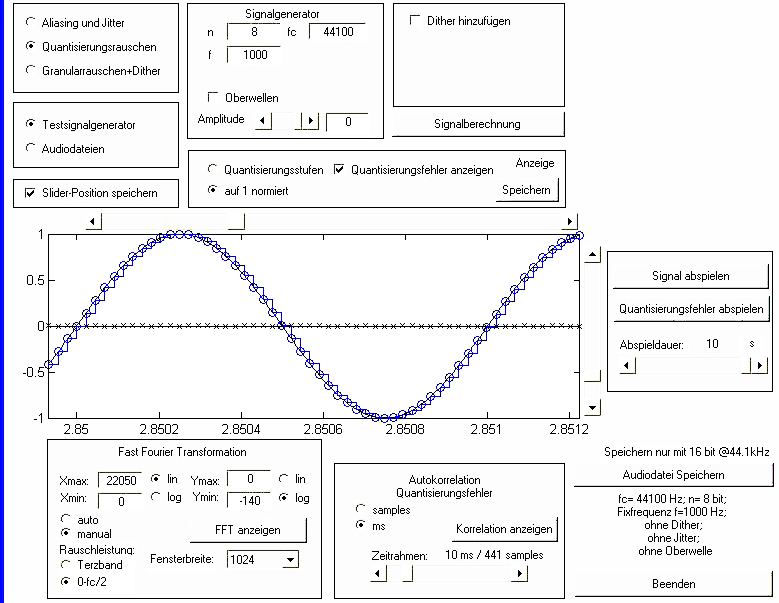
\includegraphics[width=\columnwidth]{figures/Aufg1/2_1_1.JPG} 
\caption{Darstellung eines Signales mit $f_S = 1000Hz$ und des Quantisierungsfehler (schwarze Kreuze) bei 8 Bit Wortbreite und Vollaussteuerung.}
\end{figure}

\begin{figure}[h!]
\centering
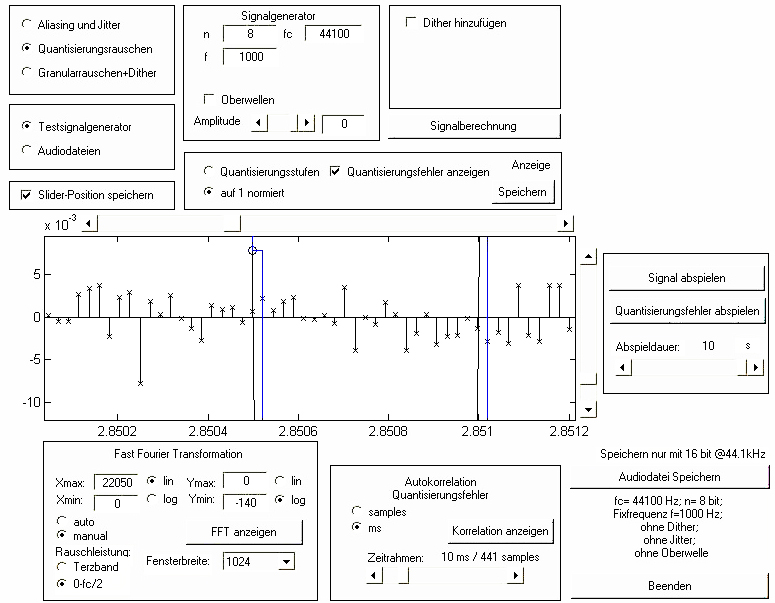
\includegraphics[width=\columnwidth]{figures/Aufg1/2_1_3.JPG} 
\caption{Darstellung des Quantisierungsfehlers und dessen Größenordnung.}
\end{figure}

\begin{figure}[h!]
\centering
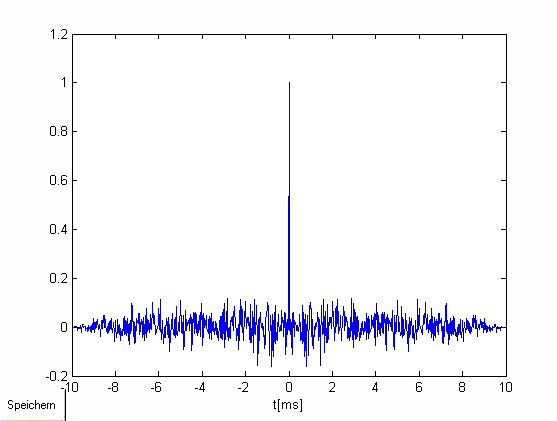
\includegraphics[width=\columnwidth]{figures/Aufg1/2_1_korr.JPG} 
\caption{Korrelation des Quantisierungsfehlers mit dem Signal.}
\end{figure}

\begin{figure}[h!]
\centering
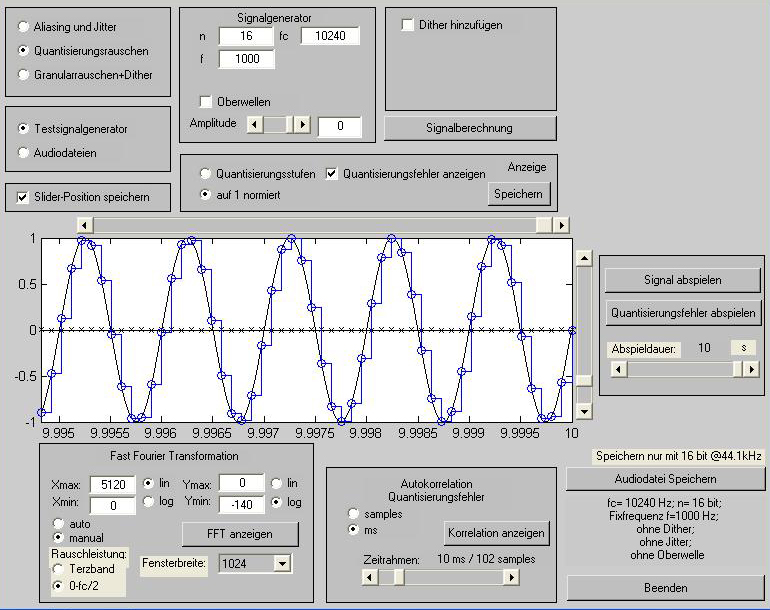
\includegraphics[width=\columnwidth]{figures/Aufg1/2_2_fenster_ok_einstell.JPG} 
\caption{Darstellung der Einstellungen und des Signals im Zeitbereich für eine FFT mit passender Fensterbreite.}
\end{figure}

\begin{figure}[h!]
\centering
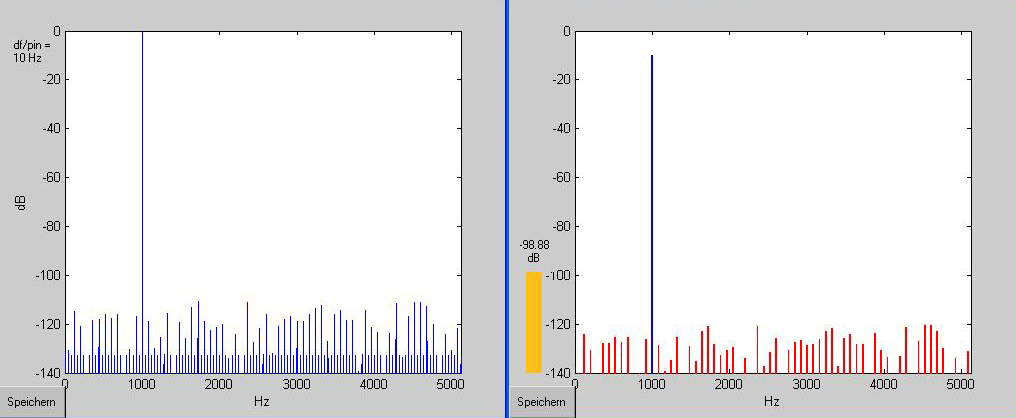
\includegraphics[width=\columnwidth]{figures/Aufg1/2_2_fenster_ok.JPG} 
\caption{Amplitudenspektrum bzw. Leistungsdichteverteilung des Signals mit Quantisierungsrauschen. Berechnet mittels FFT, einer Fensterbreite von $N = 1024$ und einer Signalfrequenz eines ganzen Vielfachem von $\frac{f_C}{N}$ ($f_S = 100 \cdot \frac{f_C}{N} = 100 \cdot \frac{10240}{1024} = 1000Hz$)}
\end{figure}

\begin{figure}[h!]
\centering
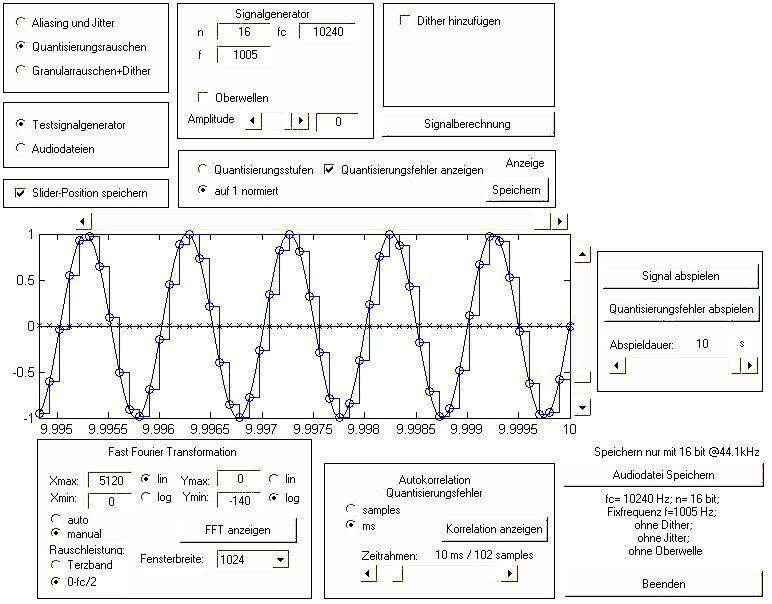
\includegraphics[width=\columnwidth]{figures/Aufg1/2_2_fenster_schlecht_einstell.JPG} 
\caption{Einstellungen und Signal im Zeitbereich für eine FFT mit möglichst starkem Lattenzauneffekt.}
\end{figure}

\begin{figure}[h!]
\centering
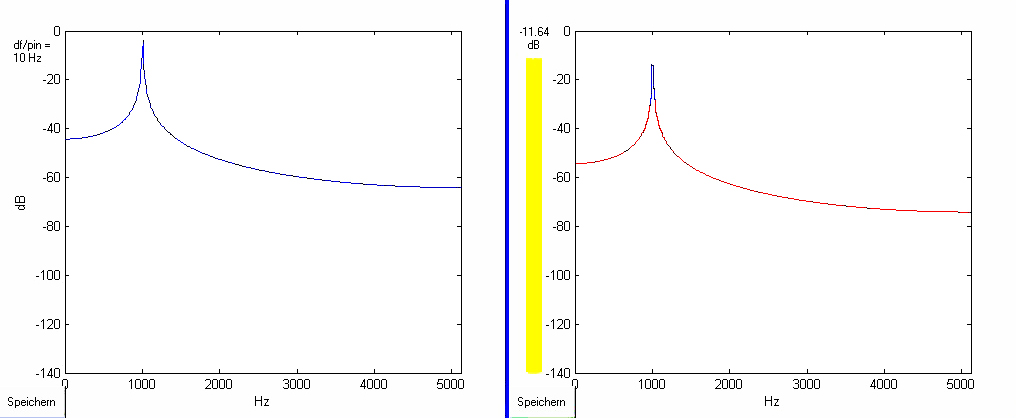
\includegraphics[width=\columnwidth]{figures/Aufg1/2_2_fenster_schlecht.JPG} 
\caption{Amplitudenspektrum bzw. Leistungsdichteverteilung des Signals mit Quantisierungsrauschen. Berechnet mittels FFT, einer Fensterbreite von $N = 1024$ und einer Signalfrequenz für möglichst starkem Lattenzauneffekt $f_S = 100.5 \cdot \frac{f_C}{N} = 100.5 \cdot \frac{10240}{1024} = 1005Hz$}
\end{figure}

\begin{figure}[h!]
\centering
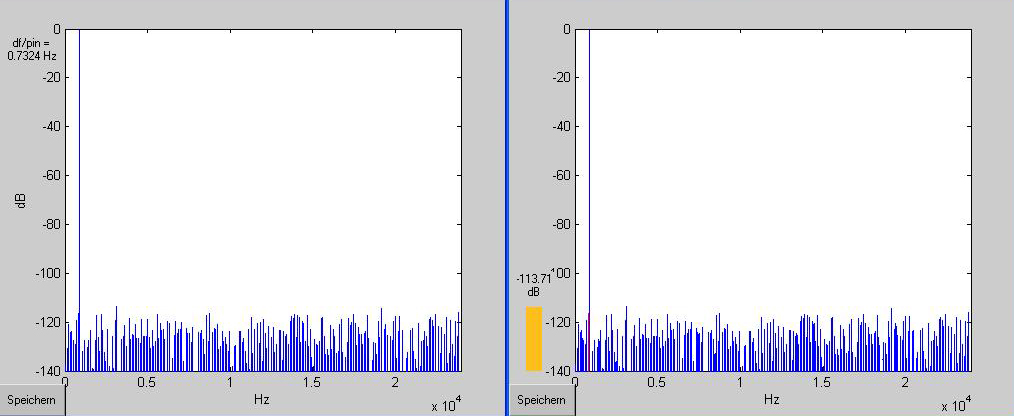
\includegraphics[width=\columnwidth]{figures/Aufg1/2_3_890hz.JPG} 
\caption{Amplitudenspektrum bzw. Leistungsdichteverteilung und Rauschleistung eines Signals mit Quantisierungsrauschen ($f_C = 48000Hz$, $f_S = 890.625Hz$).}
\end{figure}

\clearpage

\subsubsection{Diskussion}

%-------------------------------------------------------------------------------
%
% Granularrauschen und Dither
%
%-------------------------------------------------------------------------------

\subsection{Granularrauschen und Dither}
Diese Unterübung wurde aus Zeitgründen nur mündlich mit dem Laborbetreuer erarbeitet. 

\subsection{Geräteliste}
\begin{itemize}
\item Computer
\item Lautsprecher
\end{itemize}
